\setchapterpreamble[u]{\margintoc}
\chapter{Databases}
\epigraph{\emph{"It is a capital mistake to theorize before  \\ one has data."}}{ -- Sherlock Holmes}

As of the time of this writing, humanity has created nearly 100 zettabytes\sidenote[][*8]{That is, $8 \times 10^{21}$ bits. To put that into perspective, the typical hard drive is 1 terabyte in size. It would take 100 billion of these to store all of this data.} of digital data. Strongly tied to recent developments in Internet of things and machine learning, familiarity with data storage is a useful tool for any developer. But before delving into the methods and challenges associated with storing data, it's important to fully address why external data storage is so useful.

To do so, we can consider an analogy of a restaurant serving breakfast. Let's assume a new customer enters the restaurant, orders some eggs and bacon, and sits down to eat. The waiter then communicates this order to the kitchen, where a low ranking cook will rush to gather the eggs and bacon required from the fridge in order to prepare the dish. A second customer then enters and attempts to order some eggs, only to be told by the waiter that the restaurant is short on supplies. Why might this be the case? Sharp readers will know that it's likely that the last of the eggs in the fridge were used to make the first customer's dish! In this scenario, the fridge represents our \kw{database}, the eggs represent our \kw{data}, and the restaurant dining room along with the customers inside represent our web application. From this example, we note that creating a shared supply of data for many users necessitates an external database to keep things consistent between them. Just as it's not possible for a restaurant to simultaneously \emph{have} and \emph{not have} eggs in their fridge, we need to keep the data for our web app in a centralized location to allow for a degree of consistency.

In addition to facilitating a shared experience between users, aggregating data in a database solves another issue: data persistence. \kw{Data persistence} refers to the concept of any changes made by a user in an application continuing to exist, even if the application is closed or restarted. We can liken this to a customer entering a restaurant and buying their last ham sandwich on Monday, then returning on Tuesday to find the restaurant out of ham. The change made to the state of the restaurant persists into the next day, ensuring continuity in the customer's experience.\sidenote{Even though it may not be what the customer was hoping to see upon arrival.} Databases can be utilized to accomplish this in the context of a web app.

With a strong motivation for utilizing a database, let's delve deeper into what databases actually store, common implementations, and how to interact with them. 

% \margingraphic{Database.png}{The classic shorthand representation of a database, a stack of cylindrical disks }

\section{Spreadsheets and Schemas}

Databases can be as simple as a set of flat files in our file system. Assuming our web application has read and write access to our files\sidenote{Giving a program read access to a file allows it to view its contents while write access allows it to modify the contents of the file.}, we can persist any changes even if our web application has closed. However, this implementation can be challenging to work with and is a bit more granular that we will need for our tech stack.\sidenote{Fun fact: up until about 15 years ago, UCLA kept all student records in flat files. However, this system had many issues due to poor data integrity and inconsistencies, leading to a switch to a more traditional database.} Instead we will begin by considering its cousin, the \kw{spreadsheet}. A spreadsheet is a file with columns and rows - effectively a large table.\sidenote[][*5]{You can actually generate these without using any external libraries. Try to think how you might encode a table and its data in a text file.} In our examples we treat each row as an individual entry in our table, and recognize each column as a a unique property of our data. Common examples of spreadsheet file types are the comma separated file format (.csv), and Microsoft Excel's various formats (.xls, .xlsx, .xlsm).

% \margingraphic{Spreadsheet.png}{A simple spreadsheet made with Microsoft Excel}

\begin{center}
    \begin{tabular}{ |c|c|c| } 
        \hline
        \textbf{Item} & \textbf{Quantity} & \textbf{Price} \\ 
        \hline
        Lettuce & 20 & 3 \\ 
        \hline
        Tomatoes & 20 & 3 \\ 
        \hline
        Broccoli & 30 & 4 \\ 
        \hline
        Carrots & 80 & 3 \\ 
        \hline
    \end{tabular}
\end{center}

Let's refer back to our previous restaurant scenario. Now, instead of walking into the fridge to find and keep track of any raw ingredient, the restaurant chef can look at a note posted on the fridge that lists each item contained within. The table above displays a simple example of such a note. The set of column headers\sidenote{In this case: Item, Quantity, Price.} for this table is known as the table \kw{schema}, representing the data type and name associated with the values along each row in the table.

As the kitchen staff remove items from the fridge to fulfill orders, we expect the quantity fields of our fridge table to decrease. Likewise, when the restaurant receives a fresh shipment of groceries we expect the associated quantity fields to increase. On the off chance that new ingredients are required, additional rows can be added to the table to display the appropriate properties for that ingredient.

\begin{kaobox}[title=Getting Meta...]
    In addition to the data we've elected to store, most modern databases have options to include additional columns in a table's schema known as metadata. \kw{Metadata} refers to "data about data," and most commonly appears as a creation or modification timestamp and username, or a version id. The table below shows additional columns \texttt{Last\_Updated} and \texttt{Update\_By}, both of which are considered metadata.

    \begin{center}
        \begin{tabular}{ |c|c|c|c|c| } 
            \hline
            \textbf{Item} & \textbf{Quantity} & \textbf{Price} & \textbf{Last\_Updated} & \textbf{Update\_By} \\ 
            \hline
            Lettuce & 20 & 3 & 12/25/2022 & James \\ 
            \hline
            Tomatoes & 20 & 3 & 1/3/2023 & Nathan \\ 
            \hline
            Broccoli & 30 & 4 & 1/5/2023 & Nareh \\ 
            \hline
            Carrots & 80 & 3 & 12/20/2022 & Kevin \\ 
            \hline
        \end{tabular}
    \end{center}
\end{kaobox}


\section{Relational Databases and SQL}

The most widely used form of a database is known as a \kw{relational database} - one or more tables each with a fixed schema. This builds upon our previous model of a spreadsheet file and instead now makes use of an application to optimize data retrieval and modification, while still having the underlying representation. A defining feature of all relational databases is their guarantee to be \kw{ACID} compliant, with ACID being an acronym:

\begin{itemize}
    \item Atomic: Any operation either fully succeeds or fails and leaves the database unchanged
    \item Consistent: Any operation to modify data will leave data in a valid state
    \item Isolated: Any operation is carried out fully independently of any other operation
    \item Durable: Any operation, once successful, will be persisted in the database.
\end{itemize}

ACID compliance eliminates common issues stemming from concurrent reads and writes to a single table, and ensures the database is always in a valid state\sidenote{When working with an ACID compliant database, we can often run many operations as a single transaction, ensuring our data can be reverted if our operation fails in the middle.}. Another key feature shared by most popular relational databases is their use of \kw{Structured Query Language (SQL)} to interface with the database.

\begin{kaobox}[title=Working with SQL]
    SQL is the language of choice for nearly all relational databases, offering a way to view, edit, and delete data. Note that we won't be using it in our app's implementation, but its good to be familiar with it for the future. Assuming our table in our database is named "Fridge", below is an example query that generates the following table.

    \begin{verbatim}
    SELECT Item, Quantity, Price FROM Fridge
    \end{verbatim}

    \begin{center}
        \begin{tabular}{ |c|c|c| } 
            \hline
            \textbf{Item} & \textbf{Quantity} & \textbf{Price} \\ 
            \hline
            Lettuce & 20 & 3 \\ 
            \hline
            Tomatoes & 20 & 3 \\ 
            \hline
            Broccoli & 30 & 4 \\ 
            \hline
            Carrots & 80 & 3 \\ 
            \hline
        \end{tabular}
    \end{center}

    To select all columns in our table we simply need to specify the remaining columns, or make use of the wildcard operator, (*), which is shorthand for all columns in the table.

    \begin{verbatim}
    SELECT * FROM Fridge
    \end{verbatim}
    \begin{center}
        \begin{tabular}{ |c|c|c|c|c| } 
            \hline
            \textbf{Item} & \textbf{Quantity} & \textbf{Price} & \textbf{Last\_Updated} & \textbf{Update\_By} \\ 
            \hline
            Lettuce & 20 & 3 & 12/25/2022 & James \\ 
            \hline
            Tomatoes & 20 & 3 & 1/3/2023 & Nathan \\ 
            \hline
            Broccoli & 30 & 4 & 1/5/2023 & Nareh \\ 
            \hline
            Carrots & 80 & 3 & 12/20/2022 & Kevin \\ 
            \hline
        \end{tabular}
    \end{center}

    Now considering the case of a chef removing items from the fridge to prepare a meal, we make use of SQL's \texttt{UPDATE} and \texttt{WHERE} keywords, which lends itself to the following syntax. Note the single equal sign = acts as an assignment operator after the \texttt{SET} keyword, but ordinarily performs an equality comparison. We also see that SQL's string type is called \texttt{VARCHAR}, referring to a variable length character field, and must be quoted with single quotes. The query below will subtract 1 from the carrot and lettuce quantity fields.

    \begin{verbatim}
    UPDATE Fridge
    SET Quantity = Quantity - 1
    WHERE Item = 'Carrots' OR Item = 'Lettuce'
    \end{verbatim}
    
    Finally, to add a new ingredient to our table, we can make use of the \texttt{INSERT} SQL operation. In the case of adding a single row we choose to use the \texttt{VALUES} variant, but can opt to use the \texttt{SELECT} variant if adding multiple rows. To set the \texttt{Last\_Updated} metadata field, we make use a database specific date function (\texttt{CURDATE()} is built into MySQL). When designing our table, it would be best practice to provide this function as the default value for the Last\_Updated column.

    \begin{verbatim}
    INSERT INTO Fridge (Item, Quantity, Price,
    Last_Updated, Updated_By)
    VALUES (
        'Spinach',
        100,
        2.5,
        CURDATE(),
        'ACM Hack'
    )
    \end{verbatim}
    
    After all of our queries, we are left with the following table.

    \begin{center}
        \begin{tabular}{ |c|c|c|c|c| } 
            \hline
            \textbf{Item} & \textbf{Quantity} & \textbf{Price} & \textbf{Last\_Updated} & \textbf{Update\_By} \\ 
            \hline
            Lettuce & 19 & 3 & 12/25/2022 & James \\ 
            \hline
            Tomatoes & 20 & 3 & 1/3/2023 & Nathan \\ 
            \hline
            Broccoli & 30 & 4 & 1/5/2023 & Nareh \\ 
            \hline
            Carrots & 79 & 3 & 12/20/2022 & Kevin \\ 
            \hline
            Spinach & 100 & 2.5 & 1/9/2023 & ACM Hack \\
            \hline
        \end{tabular}
    \end{center}
    
    Fortunately SQL has a very gradual learning curve for its fundamental features, making it relatively simple to jump into using it!
\end{kaobox}

Beyond these features, relational databases support more advance table configurations such as constraints,\sidenote{Adding constraints to our database allows us to catch human errors before they snowball into larger issues} primary keys, and foreign keys. It is from these features - specifically the ability to enforce relationships between different schema fields and tables - that this type of database derives its name. Below are the five most popular relational databases

\begin{enumerate}
    \item Oracle
    \item MySQL
    \item Microsoft SQL Server (MSSQL)
    \item PostgreSQL
    \item IBM DB2
\end{enumerate}

\section{Non-Relational Databases}

An alternative (and a better choice in certain scenarios) is a \kw{non-relational database}, frequently referred to as a \kw{NoSQL database}\sidenote{Some non-relational databases can be queried with SQL and SQL like languages, but most are intended to be interacted with directly through code.}. Like the name implies, non-relational database are structured differently from their relational counterparts. 

\subsection*{Non-Relational Storage}

A key distinguishing feature of a non-relational database is its lack of a rigid schema and of tables altogether. Instead we store each record of data either as a \kw{document} or a \kw{key-value pair}. To understand the meaning and motivation behind this storage method, let's return to our restaurant scenario. Instead of displaying a table on our Fridge with information about our raw ingredients, let's instead display each ingredient on its own distinctly colored sticky note, like in Figure 2.1.

\margingraphic{NoSQLDiagram.png}{A visual representation of a non-relational database}

This representation aligns closely with a non-relational database, with each sticky note being analogous to a single document in our database. Note that although in our example, each sticky note contained the same fields, we could add additional fields as desired. We can call a set of documents in a non-relational database a \kw{collection}, a concept akin to a table in a relational database.

Now imagine when the chef of our restaurant has been using this sticky note system for the last couple months and has gotten very used to it - so much so that they simply consider the sticky note color and quantity value before removing the relevant ingredients they need. Here, the sticky note color parallels the concept of a unique id field associated with each document. Similar to the chef's instinctive association of a particular color with a particular document, a non-relational database makes use of a \kw{hash function} to map a document id to a particular document. Although the exact mechanics of these hash functions\sidenote{Hash functions are generally are implemented with hardware or optimized and concise software and map a unique set of input into a unique id.} are beyond our scope, they efficiently associate an id with a document, providing the backbone for fast operations in a non-relational database. For those familiar with the concept (or those planning to take CS 32 in the future), this makes our collection a variant of a \kw{hash table}.

\subsection*{Recording Documents: JSON}

In most non-relational databases (including MongoDB\sidenote{The 'M' in MERN stands for "MongoDB" - a popular non-relational database}) documents are written using the JavaScript Object Notation or \kw{JSON}. JSON syntax attempts to provide an efficient way to list a series of key value pairs. Below is a small piece of JavaScript code that would represent the lettuce document in our restaurant example. 

\begin{lstlisting}[language=Java]
    lettuce = {
        _id: 00000123456879,
        __v: 0,
        item: "Lettuce",
        quantity: 20,
        price: 3,
    }
\end{lstlisting}

As the name implies, JSON is just a way of encoding a Javascript object as a string. We can encode the object above as follows\sidenote{Note that a single JSON string corresponds to a single object (though we can group multiple together by nesting objects)}:

\begin{lstlisting}[language=Java]
    {
        "_id": 00000123456879,
        "__v": 0,
        "item": "Lettuce",
        "quantity": 20,
        "price": 3
    }
\end{lstlisting}

In our example above, the syntax for each key-value pair is to separate the two with a colon and to comma separate each entry in any given document. The metadata fields included begin with an underscore to signify they are special fields (although the specific format will depend on the database being used). As we will see when constructing our app, modifications and additions to our data will also be formatted in JSON.

The five most popular non-relational databases currently used are as follows

\begin{enumerate}
    \item MongoDB
    \item Redis 
    \item Elasticsearch
    \item DynamoDB
    \item Neo4j
\end{enumerate}

\section{Selecting and Hosting a Database}

Although we've elected to use MongoDB, a popular non-relational database as a part of the established MERN tech stack, we will briefly discuss the advantages of each type of database and how to host them. Below are the main advantages of using a relational database

\begin{itemize}
    \item Integrity: constraints on data can be easily set and enforced
    \item Reliability: simple and efficient to backup data
    \item Security: decades of strong and reliable storage methods
    \item ACID Compliant: any operation on the database will be Atomic, Consistent, Isolated, and Durable
    \item Transactable: can perform a series of complex operations as a single transaction (good for Online Transaction Processing  - OLTP\sidenote{Whereas an OLTP use case aligns well with a relational database, a non-relational database will likely also perform well. For Online Analytical Processing (OLAP) - performing analysis on very large datasets - a better choice would be a relational data warehouse.})
    \item Programmability: can define stored procedures and functions to streamline queries 
\end{itemize}

Non-relational databases provide the following advantages

\begin{itemize}
    \item Scalability: can scale storage size and compute power
    \item Open Source: source code of common databases can be analyzed and understood
    \item Efficient: can perform queries faster than relational databases
    \item Data Complexity: can store complex data types
    \item Simplicity: simple configuration and maintenance 
\end{itemize}

As we expect to have a small number of users, would prefer a faster configuration, are not really concerned with ACID compliance or security, and would like efficient code, we choose to use a non-relational database. 

It is also important to consider the computer we will run our database on. If a single developer is designing a database, it is possible to run most types of databases locally on Windows, Linux, or MacOS, saving the underlying data on your computer's local disk. Under this setup, the database will be inaccessible when the computer has been shut down, making development by other collaborators challenging. 

An alternative to hosting a database on your computer may be running the database on a dedicated computer you can guarantee will be continuously running. After configuring the connection between your web application and database computer,\sidenote{A computer used to run a database in this way is commonly called a database server. We'll talk  more about servers in chapter 3.} we alleviate the issue of having our data continuously available, but introduce a new issue: we must now maintain a distinct computer dedicated for our database.

A popular alternative that facilitates collaboration is to run the database on a third-party computer with the power of \kw{cloud computing}. Most major cloud service providers offer free storage options, enabling users to run and access a database on a computer in one of their warehouses. To make this process simpler, MongoDB has partnered with AWS, Azure and Google Cloud to offer their \kw{MongoDB Atlas}. By creating a \href{https://www.mongodb.com/cloud/atlas/register}{MongoDB Atlas account}, one can easily create a database on the cloud, and connect to it from in the browser, through the command line, or through code.

\section{Mongoose and Asynchronous Programming}

The final step of using our hosted database is writing some code to access and manipulate our database. Here we will take advantage of a programming library to make our job a bit simpler. 

\subsection*{Using Mongoose}

In our restaurant analogy, let's assume there is one kitchen worker named Cameron whose sole job is to retrieve ingredients from the fridge (which can be quite complicated due to its size and eccentric method of organization). Without Cameron, each chef would be required to learn how to navigate this unwieldy fridge in order to get the ingredients required for a recipe. Thankfully, Cam is here to shoulder the burden. In our MERN tech stack, Cameron is akin to the \kw{mongoose} library, a JavaScript Object Data Modeling library for MongoDB that simplifies the process of retrieving and modifying data in our database. 

Using mongoose allows us to define an expected schema for the documents in our collection. Let's consider what creating a schema for our documents in our restaurant scenario would look like. First, we must signify our intention to use mongoose, done in the first line of the below code. We then define a new Schema, with each intended data field mapping to its relevant data type and properties. Finally, we choose to export our newly defined model so we can use it in future files.

\vspace{.5cm}

\begin{lstlisting}[language=Java]
    const mongoose = require('mongoose');

    const ingredient = new mongoose.Schema({
            item: {
                type: String,
                required: true
            },
            quantity: {
                type: Number,
                required: true
            },
            price: {
                type: Number,
                required: true
            }
    });

    module.exports = mongoose.model('Ingredient', ingredient);
\end{lstlisting}

The schema above corresponds to a Javascript object of the following form:

\begin{lstlisting}[language=Java]
    ingredient = {
        item: "beef",
        quantity: 21,
        price: 5
    }
\end{lstlisting}

Mongoose also offers a wide variety of intuitive functions to manipulate and add new documents to the collection with a particular schema.\sidenote{These functions are part of mongoose's Application Programming Interface (API). An API is simply a term used to describe an interface to take advantage of the features of a programming library, application, or framework.} Below is a short list of some of the most commonly used functions, the most relevant of which we will use in our demo.

\begin{itemize}
    \item \texttt{Model.findById()}: Finds a single document by its \_id field.
    \item \texttt{Model.findByIdAndDelete()}: Finds a single document by its \_id field and deletes it.
    \item \texttt{Model.findByIdAndUpdate()}: Finds a single document by its \_id field and updates it.
    \item \texttt{Model.find()}: Finds documents matching certain fields. A more general form of \texttt{findById()}.
    \item \texttt{Model.create()}: Creates a new document.
    \item \texttt{Model.count()}: Counts number of documents that match an object in a collection.
\end{itemize}

\subsection*{Asynchronous vs Synchronous}

In order to discuss Mongoose in more depth, we must first make a slight detour and discuss a concept that may be entirely new to you: asynchronous programming.\sidenote{Or maybe not. But it's still important to understand asynchronous programming in depth, so stick with us!} Yet again, let's go back to the the restaurant scenario, this time considering a chef, Manny, preparing a dish: ramen with veggies! Veggie ramen is relatively simple to make, but there are a couple of steps one needs to follow:

\begin{enumerate}
    \item Boiling Water
    \item Adding Ramen
    \item Cutting Veggies
    \item Adding Veggies
\end{enumerate}

Let's say boiling water takes three minutes and cutting your vegetables takes two. Each of the other steps only takes a handful of seconds, which is neglible for this context. Starting with step 1 and ending with step 4, it would take Manny a total of five minutes to finish preparing the ramen. This is \emph{decent}, but Manny works at a Michelin Star restaurant and he has a reputation to uphold! Rather than doing everything sequentially, he notices that some of the steps are independent of each other and can be done at the same time.\sidenote{Namely, boiling water and cutting veggies.} With this insight in mind, Manny sets the water to boil and soon after starts cutting the veggies. He finishes cutting the veggies after 2 minutes, and sets them aside. A minute later the water finishes boiling, and so he adds the ramen and the veggies to the pot. Voila! Manny shaved a whole two minutes off of his preparation by deciding to perform some of the steps \emph{at the same time}. 

These two methods of preparation respectively represent synchronous and asynchronous methods of programming! Take a look at the visualization below for a clearer idea of the concept.

\begin{center}
    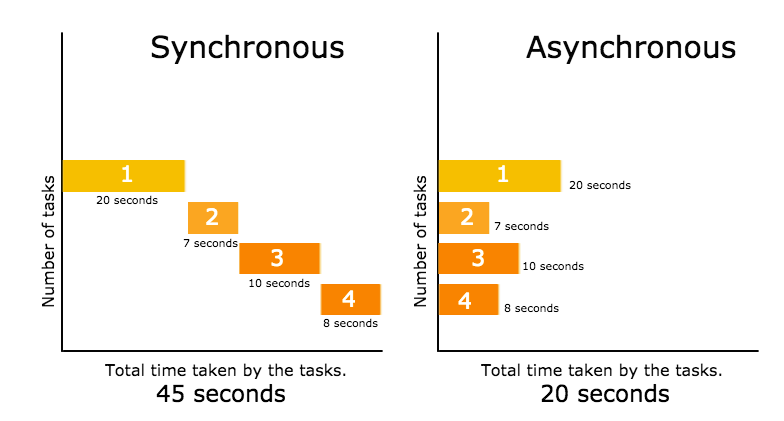
\includegraphics{SyncvsAsync.png}
\end{center}

Unless otherwise indicated, most of the code you write is synchronous. That is, if there are any tasks that take a long time to complete,\sidenote{Such as getting a lot of data from a database \emph{cough cough}.} they may serve as a bottleneck to other, potentially unrelated tasks. As you might expect, we can get around this with asynchronous programming. 

\subsubsection*{Taking things slowly...}
Continuing with our analogy, let's write some code that represents the situation. Suppose we have a function for each task mentioned above.

\begin{lstlisting}[language=Java]
    const boilWater = () => {
        // implemenation details here
        // ALWAYS TAKES 3 MINUTES
        // logs to console when finished
    };

    const addRamen = () => {
        // implemenation details here
        // INSTANT, but can only be done after water finishes boiling
        // logs to console when finished
    };

    const cutVeggies = () => {
        // implemenation details here
        // ALWAYS TAKES 2 MINUTES
        // logs to console when finished
    };

    const addVeggies = () => {
        // implemenation details here
        // INSTANT, but can only be done after water finishes boiling
        // logs to console when finished
    };
\end{lstlisting}

The synchronous approach is as follows and, as noted before, will take five minutes to complete.

\begin{lstlisting}[language=Java] 
    boilWater(); // 3 minutes
    addRamen();
    cutVeggies(); // 2 minutes
    addVeggies();
\end{lstlisting}

How can we do better? Introducing promises! \kw{Promises} are objects in Javascript that "represent the eventual completion (or failure) of an asynchronous operation, and its resulting value." In (slightly) more concrete terms, they are wrappers for values that might not yet be determined, which is typical of asynchronous code. Consider the \texttt{boilWater()} function. Below is an idea of what an asynchronous version of the function might look like in Javascript.\sidenote{The syntax may seem a bit strange upon first glance and admittedly, it is. The good news is that in the context of this series, this is the only time we will write asynchronous code this way. So don't worry if this is a bit confusing to you!} 

\begin{lstlisting}[language=Java] 
    const boilWater = () => {
        return new Promise((resolve, reject) => {
            // implemenation details here
            // ALWAYS TAKES 3 MINUTES
            // logs to console when finished
        });        
    };
\end{lstlisting}

We can do the same for our other intensive task, \texttt{cutVeggies()}. Now, when we call either of these functions, it won't halt the rest of our code!

\begin{lstlisting}[language=Java] 
    boilWater(); // 3 minutes
    addRamen();
    cutVeggies(); // 2 minutes
    addVeggies();
    // in total, will only take 3 minutes... but there's a problem.
\end{lstlisting}

Unfortunately, we have an issue. As the code is currently written, we do not distuinguish dependent and independent tasks. This means that we will end up adding pasta to our water before we finish boiling and we'll add our veggies before we finish cutting. How can we handle this? We'll show two equally viable ways.


1. Using \texttt{.then()}
\begin{lstlisting}[language=Java] 
    cutVeggies(); // 2 minutes
    boilWater().then(() => {
        addRamen();
        addVeggies();
    }); // 3 minutes
    // in total, will only take 3 minutes!
\end{lstlisting}

Notice that we are passing in an \emph{anonymous function} to \texttt{.then()}, which is executed upon completion of \texttt{boilWater()}.\sidenote{When the code within a promise is completely executed, the promise is said to have been \kw{resolved.}} Now, everything works as expected. We can also write this another way, which we will actually prefer throughout this workshop series.
    
2. Using \texttt{async/await}
\begin{lstlisting}[language=Java] 
    const prepareRamen = async () => {
        cutVeggies();
        await boilWater();
        addRamen();
        addVeggies();
    };
    // in total, will only take 3 minutes!
\end{lstlisting}

Looks a bit cleaner, right? The await keyword is similar to \texttt{.then()} in that we will wait for the promise returned by \texttt{boilWater()} to be resolved before we continue in our code. Note that when using \texttt{await} we must wrap our code in a function marked \texttt{async}, otherwise we will get a syntax error. 

Thinking beyond this example, we typically utilize asynchronous code in any situation that involves many intensive independent tasks. For example, loading a 4k image. We don't want to halt our entire program to wait for the image to load, so instead we load it in the background using asynchronous programming. Now that all of that's out of the way, we can move on to actually using asynchronous programming in the context of MongoDB!

\subsection*{Mongoose Queries}

Below is a snippet of code that builds upon our mongoose schema defined in the above code sample and defines an asynchronous function. The snippet below first includes the specified model, then defines an asynchronous function to return all documents matching our defined schema using the find() function. We return these documents by setting them in the result object.

\begin{lstlisting}[language=Java]
    const Ingredient = require("../models/Ingredient");

    module.exports.getIngredients = async (req, res) => {
        const ingredients = await Ingredient.find();
        res.send(ingredients);
    }
\end{lstlisting}
    
\section{Demo}

% \section{Testing}

% \section{Organization}
